\documentclass{beamer}
\usetheme{Singapore}
\setbeamercovered{transparent}

\usepackage{ dsfont }
\usepackage{ amsmath }
\usepackage{ mathrsfs }
\usepackage{ amssymb }
\usepackage{ amsthm }
\usepackage{ graphicx }
 
\usepackage[utf8]{inputenc}

\newcommand{\Prob}{\mathbb{P}}

\AtBeginSection[]
{
	\begin{frame}
		\frametitle{Table of Contents}
		\tableofcontents[currentsection]
	\end{frame}
} 
 
 
%Information to be included in the title page:
\title{Statistical Models for Bursty Events}
%\subtitle{}
\author{Smarak Nayak}
\date{July 20, 2016}
 
 
\begin{document}
 
\frame{\titlepage}
\section{Introduction}

\begin{frame}{Motivation}
	Classical extreme value theory assumes that events happen uniformly. \\~\\
	
	However this is not always the case, in many systems the events occur in bursts. \\~\\
	
	Examples include both human-created events and physical phenomena:
		\begin{itemize}
		\item Communication
		\item Financial Trades 
		\item Network Traffic
		\item Neuron Firing Sequences
		\item Seismic Activity
	    \end{itemize}
	
\end{frame}

\begin{frame}{Example Process }
    \begin{figure}
        %\centering
        \hspace{-0.5cm}
        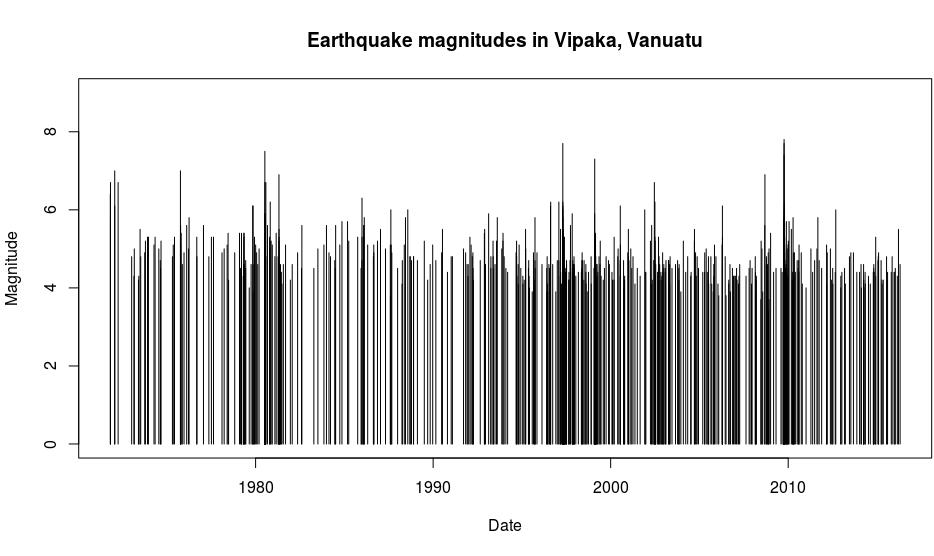
\includegraphics[scale=0.45]{EarthQuakeData.jpeg}
        %\caption{Caption}
        %\label{fig:my_label}
    \end{figure}

\end{frame}

\begin{frame}{Example Process After Thresholding}
    \begin{figure}
        %\centering
        \hspace{-0.8cm}
        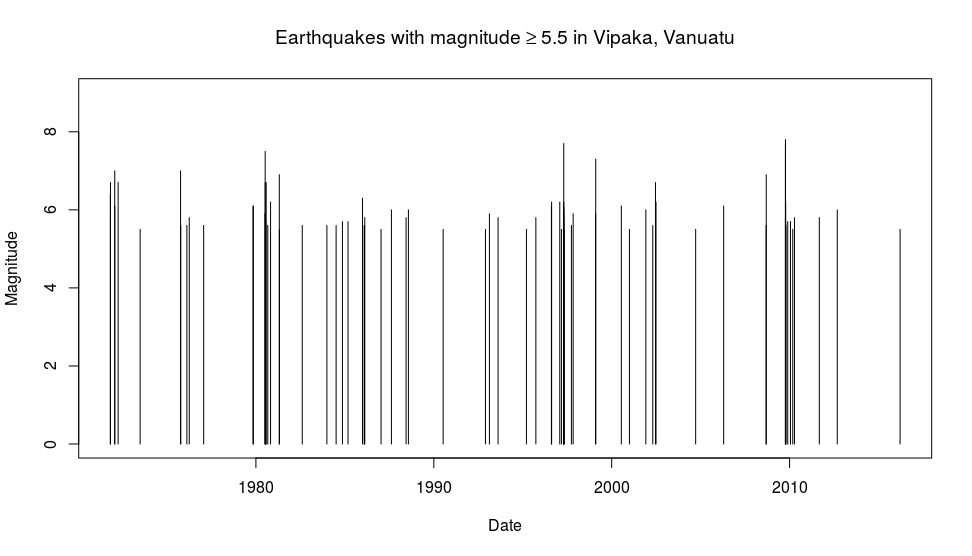
\includegraphics[scale=0.45]{ThresholdedEQData.jpeg}
        %\caption{Caption}
        %\label{fig:my_label}
    \end{figure}
\end{frame}
 
\begin{frame}{Notation}
	
	Let $J_1 , J_2 , ...$ be a sequence of i.i.d. random variables that model the jump sizes (event magnitudes).
	\\~\\
	Let $W_1, W_2, ...$ be a sequence of i.i.d positive random variables that model the waiting times between the jumps.
	\\~\\
	We can then define $(W_1 , J_1 ), (W_2 , J_2 ), ...$ to be a sequence of i.i.d $\mathbb{R} \times \mathbb{R} ^+$ random variables.
\end{frame}

\begin{frame}{Notation Contd.}
    Now define the sum of the first $n$ waiting times to be $S(n):=\sum^n_{i=1} W_i$
    \\~\\
    Define the maximum of the first $n$ jumps to be $M(n):=\bigvee_{i=1}^n J_i$
    \\~\\
    Define a renewal process $N(t):=\max\{n\geq0:S(n)\leq t\}$
    \\~\\
    Finally we define the Continuous Time Random Maxima (CTRM) to be $V(t):=M(N(t))=\bigvee_{i=1}^{N(t)} J_i$
\end{frame}

\begin{frame}{CTRM Example}
    \begin{figure}
        \centering
        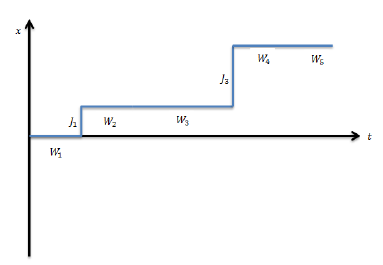
\includegraphics[scale=1]{CTRM.png}
        %\caption{Caption}
        %\label{fig:my_label}
    \end{figure}
\end{frame}

\begin{frame}{ A Possible Model }
	We first assume that the waiting times and jump sizes are independent.
	\\~\\
	Waiting times $W_i$ are modelled according to a stable distribution with stability parameter $\beta \in (0,1)$, skewness parameter 1, location parameter 0, and scale parameter =1.
	\\~\\
	Jump sizes $J_i$ are modelled according to Generalized Extreme Value (GEV) distribution with location parameter $\mu$, scale parameter $\sigma$ and shape parameter $\psi$.
	\\~\\
	The primary goal is to design methodology that fits models to data sets of bursty events.
\end{frame}

\begin{frame}{Simulated data}
    \begin{center}
        $\mu=0, \sigma=1, \psi=0.3,\beta=0.7$
    \end{center}
	\begin{figure}
        \centering
        \vspace{-0.5cm}
        \hspace{-0.8cm}
        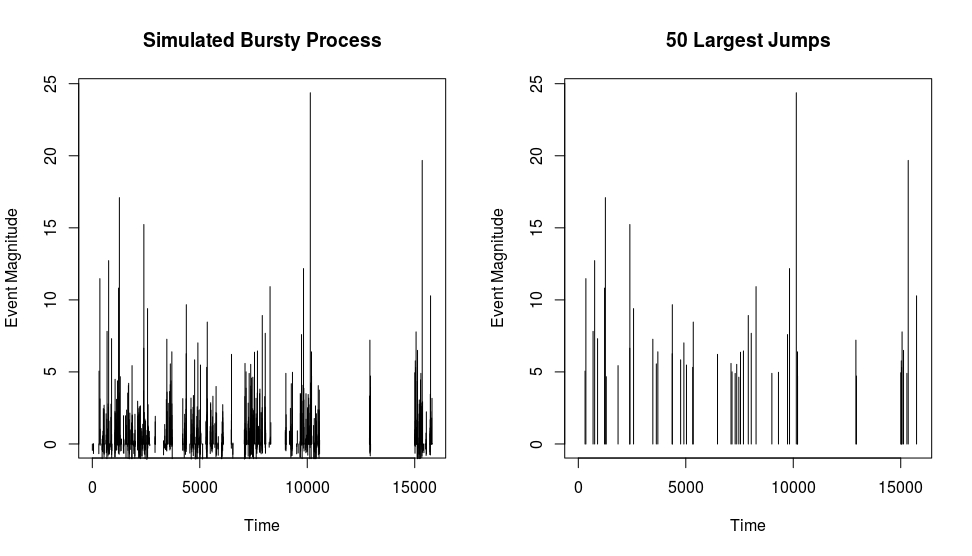
\includegraphics[scale=0.45]{SimulatedBursty.jpeg}
        %\caption{Caption}
        %\label{fig:my_label}
    \end{figure}
\end{frame}
\section{Maximum Likelihood Estimation of $\beta$}
\begin{frame}{Distribution of Durations}
    \begin{block}{Proposition (Meerschaert and Stoev (2007))}
        Let F be the cdf of a GEV random variable. Let $a$ be the threshold level, then define $T_a$ as the duration between jumps that have been thresholded at the $a$-level. Then
        \[
            T_a \sim (-\log F(a))^{\frac{-1}{\beta}}X^{\frac{1}{\beta}}D(1).
        \]
        Where $D(1)$ is a random variable of the stable distribution with stability parameter $\beta$ and skewness parameter 1 and where $X$ is a standard exponential random variable.
    \end{block}
\end{frame}

\begin{frame}{Distribution of Durations Contd.}
    After taking the logarithms of both sides we arrive at
    \[
        \log T_a \sim \frac{1}{\beta}\log X + \log D(1) -\frac{1}{\beta}\log(-\log F(a)).
    \]
    Now we have that,
    \begin{align*}
    f_{\frac{1}{\beta}\log X}(x) &= \frac{d}{dx}\Prob\left(\frac{1}{\beta}\log X\leq x\right)\\
                                 &= \frac{d}{dx}\Prob(X\leq e^{x\beta})\\
                                 &= f_X(e^{x\beta})\beta e^{x\beta}.
\end{align*}
\end{frame}

\begin{frame}{Distribution of Durations Contd.}
    We also have,
    \begin{align*}
    f_{\log D}(x)&= \frac{d}{dx}\Prob(\log D\leq x)\\
                 &= \frac{d}{dx}\Prob(D\leq e^x)\\
                 &= f_D(e^x)e^x.
    \end{align*}
    Using convolution we arrive at
    \[
    f_{\frac{1}{\beta}\log X+\log D}(x)= \int^\infty_{-\infty} f_{\frac{1}{\beta}\log X}(x-y)f_{\log D}(y)dy.
    \]
    Shifting the above expression to the right by $\frac{1}{\beta}\log(-F(a))$ gives us the density of $\log T_a$. That is,
    \[
        f_{\log T_a}(x)=\int^\infty_{-\infty} f_{\frac{1}{\beta}\log X}\left(x-y+\frac{1}{\beta}\log(-\log F(a))\right)f_{\log D}(y)dy.
    \]
\end{frame}

\begin{frame}{Distribution of Durations Contd.}
    Substituting our expressions for $f_{\log D}(x)$ and $f_{\frac{1}{\beta}\log X}(x)$ we get
    \begin{align*}
        &f_{\log T_a}(x)\\
        &=\int^\infty_{-\infty} f_X(e^{ \beta(x-y+\frac{1}{\beta}\log(-\log F(a)))})
        \beta e^{ \beta(x-y+\frac{1}{\beta}\log(-\log F(a)))}f_D(e^y)e^y dy
    \end{align*}
    which simplifies to
    \[
        f_{\log T_a}(x)=\int^\infty_{-\infty} - \log F(a) f_X(-\log F(a)e^{\beta(x-y)})\beta e^{\beta(x-y)} f_D(e^y)e^y dy.
    \]
\end{frame}

\begin{frame}{Likelihood Profile}
    The above density was used in order to calculate an MLE for the simulated data and the following likelihood profile was generated.
    \begin{figure}
        \centering
        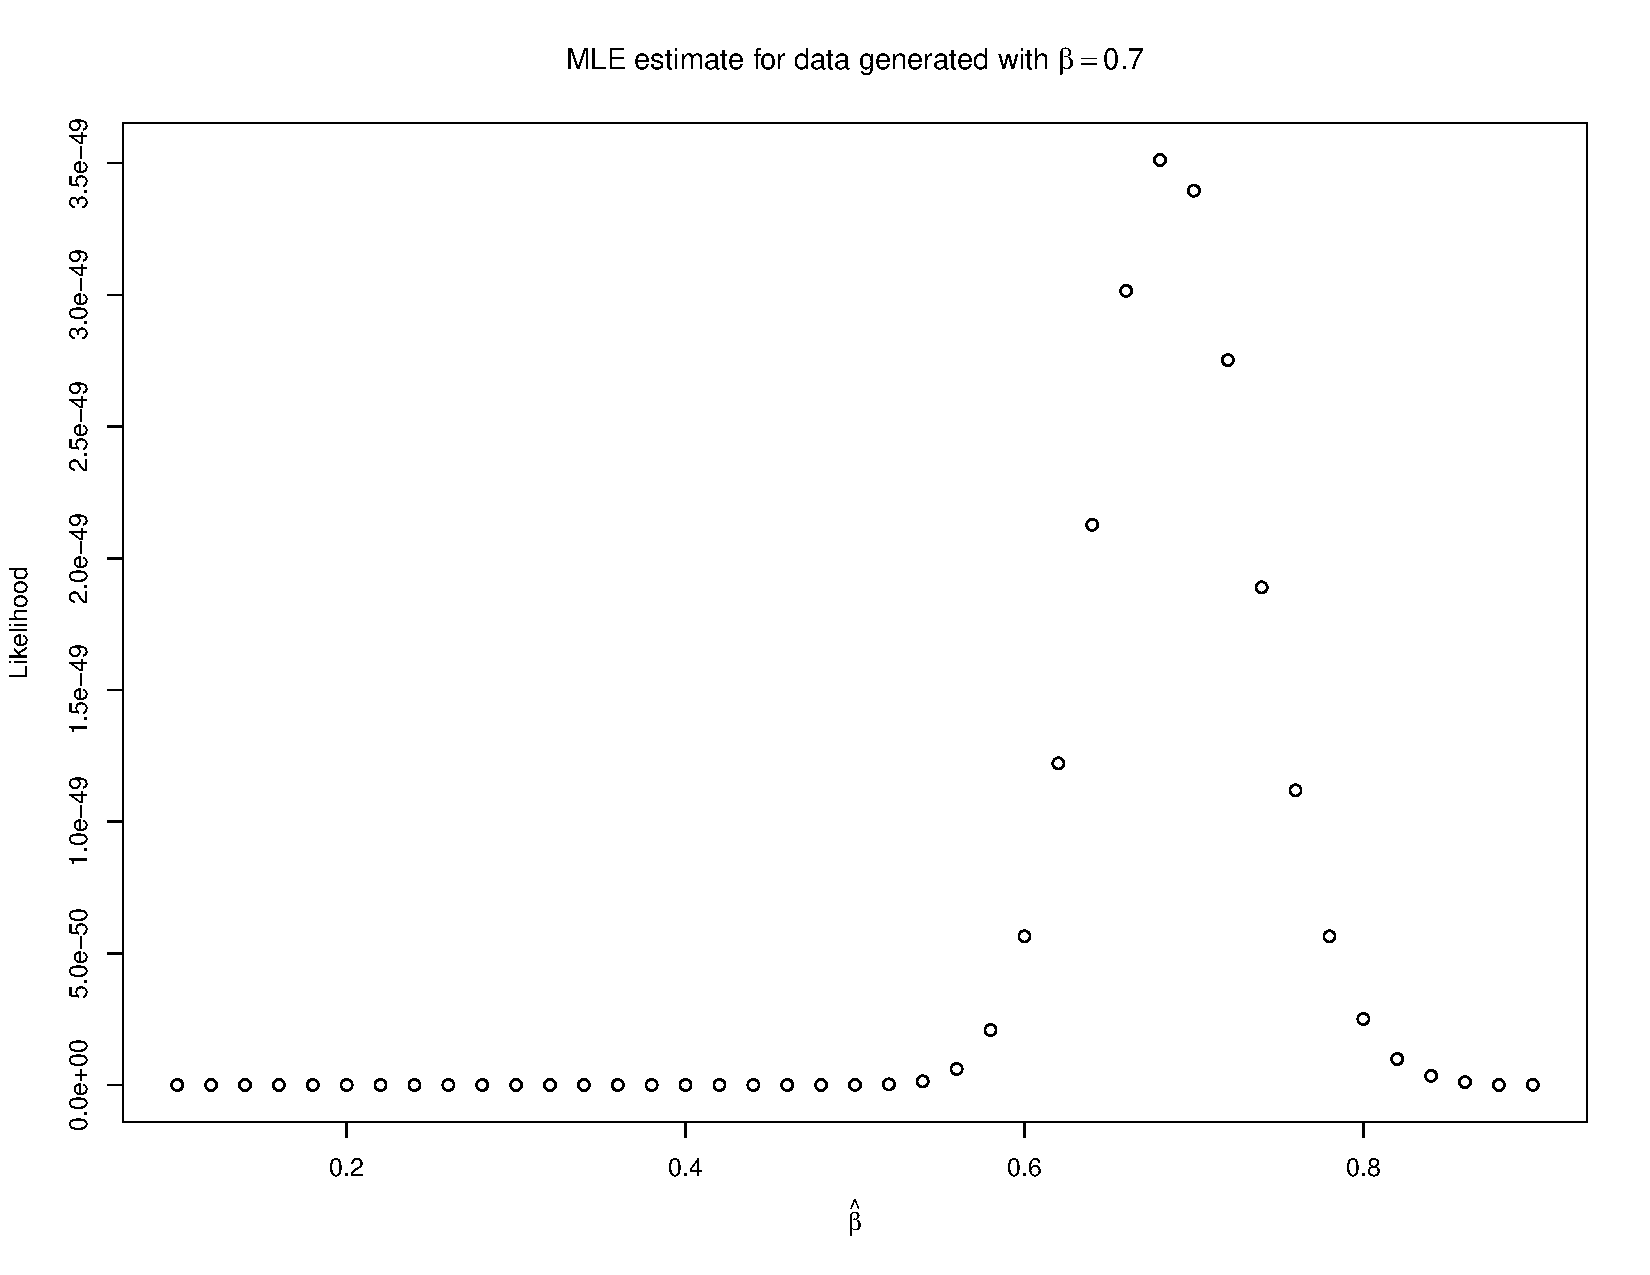
\includegraphics[scale=0.33]{LikelihoodProfile.pdf}
        %\caption{Caption}
        %\label{fig:my_label}
    \end{figure}
\end{frame}

\section{Convergence}

\begin{frame}{Convergence of Waiting Times}
	
	\begin{block}{Theorem (Meerschaert and Sikorskii (2011))}
		Suppose that $W_i$ are i.i.d. and positive with $\Prob(W_n>t)=ct^{-\beta}$ for all $t>c^{1/\beta}$, some $c>0$ and $0<\beta<1$. Then
		\[
		    n^{-1/\beta}(W_1+...+W_n) \to D \textrm{ as } n\to \infty.
		\]
		Where $D$ is distributed according to a one-sided stable distribution.
		\\~\\
	\end{block}

	This theorem can be generalised for any waiting times that follow a heavy tailed distribution (i.e mean is not finite) as follows
	\begin{equation*}
	    a_nS(n) \Rightarrow D.
	\end{equation*}
	
	
\end{frame}

\begin{frame}{Convergence of Waiting Times Contd.}
	Since we will be working in continuous time, we need to define partial processes.
	\\~\\
	Define the partial sum-process as $S(t):=\sum^{\lfloor{t}\rfloor}_{i=1} W_i$
    \\~\\
    Similarly let the partial max-process be $M(t):=\bigvee_{i=1}^{\lfloor{t}\rfloor} J_i$
    \\~\\
    \begin{block}{Theorem (Meerschaert and Sikorskii (2011))}
		Given $a_nS(n)\Rightarrow D$, where the sequence of positive constants $\{a_n\}$ is regular varying with index $-1/\beta, (0<\beta<1)$, then writing $a(t):=a_t,$
		\[
		    \{a(c)S(ct)\}_{t\geq0} \xrightarrow[c\to \infty]{J_1} \{D(t)\}_{t\geq0},
		\]
		where $\{D(t)\}_{t\geq0}$ is $\beta$-stable subordinator.
	\end{block}
\end{frame}



\begin{frame}{Convergence of Maxima}
	\begin{block}{Theorem (Lamperti (1964))}
		Recall $M(n)=\bigvee_{i=1}^n J_i$. Suppose there exists constants ${b_n}>0$ and $d_n$ such that,
		\[
		    \Prob(M_n\leq b_nx+d_n)=F^n(b_nx+d+n) \Rightarrow G(x).
		\]
		Now set
		\[
	        A^{c}(t)=
	        \begin{cases}
	            b_c(M_{\lfloor{ct}\rfloor}-d_c), &\textrm{$t\geq 1/c$}\\
	            b_c(J_1-d_c), &\textrm{$0<t<1/c.$}
	        \end{cases}
		\]
		Then $A^c \xrightarrow[c\to \infty]{J_1} A$, where $\{A(t)\}_{t\geq0}$ is an extremal process generated by G. That is
		\[
            \{b(c)(M(ct)-d(c))\}_{t\geq0} \xrightarrow[c\to \infty]{J_1} \{A(t)\}_{t\geq0}.
	    \]
	\end{block}
\end{frame}

\begin{frame}{Notation for Scaled $W_i$ and $J_i$}
    Define $W_i^c:=a(c)W_i$ and $J_i^c=b(c)(J_i-d(c))$.
    \\~\\
    Define the scaled partial sum-process as $S^c(t):=\sum^{\lfloor{ct}\rfloor}_{i=1} W_i^c$
    \\~\\
    Define the scaled partial max-process as $M^c(t):=\bigvee_{i=1}^{\lfloor{ct}\rfloor} J_i^c$
    \\~\\
    Define a renewal process $N(t):=\max\{n\geq0:S^c(n)\leq t\}$
    \\~\\
    Finally we define the scaled Continuous Time Random Maxima (CTRM) to be $V^c(t):=\bigvee_{i=1}^{N^c(t)} J_i^c$
\end{frame}

\begin{frame}{Convergence of Joint Process}
    \begin{block}{Theorem}
        Let $(W_i^c,J_i^c)$ be a sequence of i.i.d $\mathbb{R}^+\times\mathbb{R}$ random vectors such that
        \[
            \{S^c(t),M^c(t)\}_{t\geq0} \xrightarrow[c\to \infty]{J_1} \{(D(t),A(t))\}_{t\geq0}
        \]
        where the paths of $\{D(t))\}_{t\geq0}$ are non-decreasing almost surely. Then,
        \[
            \{V^c(t)\}_{t\geq0} \xrightarrow[c\to \infty]{J_1} \{(A_-\circ E)_+(t)\}_{t\geq0},
        \]
        where $E:=\inf \{u>0:D(u)>t\}$ is the inverse of $D$.
    \end{block}
\end{frame}

 
\end{document}